% !TEX TS-program = xelatex
% !TEX encoding = UTF-8 Unicode
% WORKING!!!! File encoding: UTF-8 - file need be saved as utf8
%             Latex encoding:UTF-8 - need package utf8

\documentclass[12pt]{article}
% Margins
\usepackage[a4paper]{geometry}
\geometry{verbose,tmargin=2.5cm,bmargin=2cm,lmargin=2cm,rmargin=2cm}

%==============================================================================
% Imports
%==============================================================================
% UTF-8
\usepackage[utf8]{inputenc}
% Math formulas
\usepackage{amsmath}
% Graphics
% \usepackage{graphicx} 
% Page view
\usepackage{fancyhdr}
% Matlab codes
% To use this library add mcode.sty to same folder.
% \usepackage[]{mcode}
% Subfigure caption
\usepackage{subcaption}
% Line spacing
\usepackage{setspace}
% Specific symbols (degree...)
\usepackage{gensymb}
% For function description
\usepackage{cmap}
\usepackage[T1]{fontenc}
\usepackage{times}
\usepackage[Bjarne]{fncychap}
\usepackage{longtable}
\usepackage{sphinx}
\usepackage{multirow}

%==============================================================================
% Settings
%==============================================================================
%\renewcommand{\thesection}{ \arabic{section}}
\pagestyle{fancy}
\fancyhf{}
\usepackage{titling}
\fancyhf[HC]{\thetitle}
\fancyhf[HL,HRO]{\theauthor}
\fancyhf[HR,HLO]{\today}
\fancyhf[FL,FRO]{\thepage}
% Paragraph spacing
\setlength{\parindent}{0em}
% Line spacing
\onehalfspacing

%==============================================================================
\title{Program pro měření a ukladaní dat z magnetometru}
\author{Albershteyn Andrey}

\date{\today}

\begin{document}

\maketitle

%==============================================================================
% 1
%==============================================================================
\renewcommand*\contentsname{Obsah}
\tableofcontents
%==============================================================================
% 2
%==============================================================================
\section{Description}
\par Tetno program se používá pro zprácování a ukladaní dát z observatorního
magnetometru. Cílem tohoto programu je lehký přenasitelní software pro spuštění
na jednoduchem počítače Raspberry Pi. 
\newline
\par Senzor obsahuje FPGA chip který vytváří datový stream a vysíla ho pomoci
seriového portu. Tento stream prijámeme pomoci seriového rozhraní Raspberry Pi.
\newline
\par Program je sestaven ze 3 processu. Jeden přijímá data ze seriového portu,
druhy provádí kalibrace dat a třeti ukládá data do souboru. Processy jsou
spojeny pomoci Pipeline a jsou nezávisle, jenom při ukončení hlavního processu,
který čte data, ukončujou se i vše ostatní.
\newline
\par Tento program obsahuje několik testovacích možnosti. Jednou z ních je
vysílaní impulsu při čtení dat. V konfiguračním souboru je nastaven nějaký GPIO
pin, který bude se použivat pro oznamení čtení dat, tedy před začatkem čtení a
po konci. Tento postup je užiteční pro kontrolu jsou-li přijate vše datové
vzorky.
\par Dál je možné zpustit program v Virtualním modu, což známená že budeme
testovat jenom kalibrace a ukládaní dat. Tedy nepotřebujeme žádný senzor,
protože data se budou randomě generovat přimo v programu. Tento mode je užitoční
při nějakých uprávach programu nebo ověření že všechno funguje tak jak má
fungovat.
\par Dalši možnost je použiti loggování celého cyklu vypracování dat. Program
obsahuje hlašky s potvrzeními o zpracování dat a nastavajicích chybach, které
take jde zapnout.
\newline
\par Celý program je napsat jenom s výužitim built-in python knihoven.
Takže nepotřebuje instalace nestandartních knihoven. Jenom při zapnutem Debug
oznamování (použiti nějakého GPIO pinu) je potřeba nainstalovat GPIO knihovnu
pro komunikace s piny.
%==============================================================================
% 3
%==============================================================================
\section{Program's structure}
\par V teto sekce máme popis celého programu. Tedy za co jsou odpovidní každý
soubor a jaky má funkcional. 
\par Seznam souboru:
\begin{enumerate}
    \item \textbf{main.py} - tento soubor je hlavním vstupem do programu. Běží
        jako vlastní process a provadí čtení dat ze seriového portu, které pak
        posílá do pipeline pro kalibrace.
    \item \textbf{saver.py} - obsahuje jenom jednu funkce, která je spouštěna
        jako process a provadí ukládaní dat.
    \item \textbf{calibration.py} - obshauje několik pomocních funkce, které 
        jsou použité v processore pro kalibrace a různé úpravy dat.
    \item \textbf{processor.py} - obsahuje jedinou funkce, která je spouštená
        jako process. Provadí kalibrace dat a posilá je dál do ukládacího
        processu.
    \item \textbf{reader.py} - tento soubor obsahuje funkce pro nastavnéní 
        komunikace a komunikace s zářizenim. 
    \item \textbf{generator.py} - obsahuje třidu, která slouží generatorem 
        nahodných dat použivá se jenom v Virtual modě.
    \item \textbf{settings.py} - obsahuje nastavení programu a parametry 
        kalibrace (například offsety, sensitivity atd.)
\end{enumerate}

\begin{figure}[htb!]
    \centering
    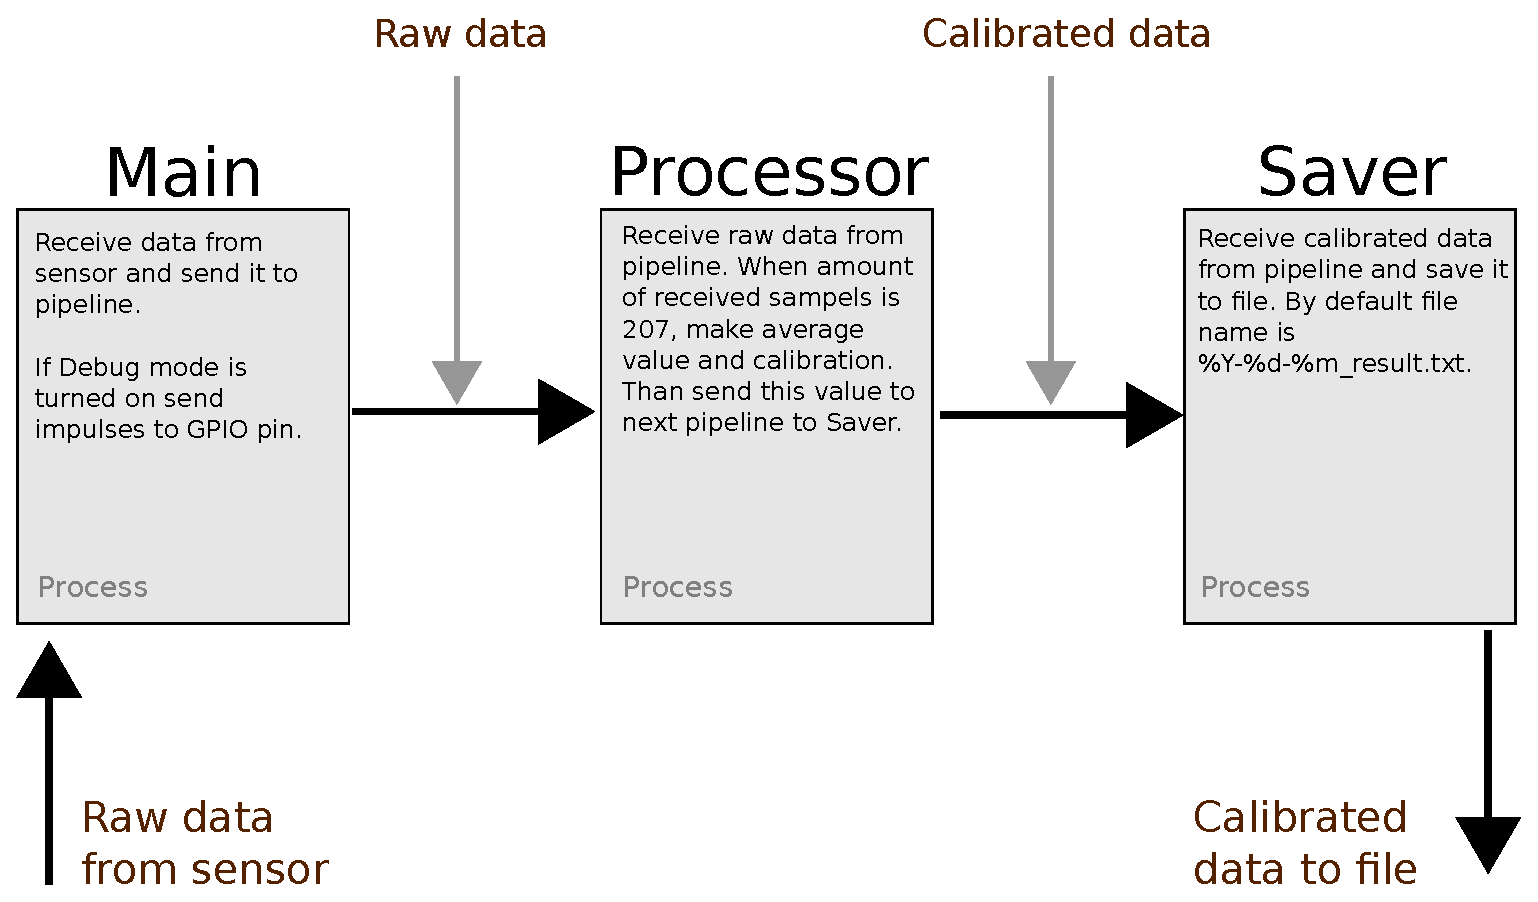
\includegraphics[width=0.7\textwidth]{./structure.eps}
\end{figure}

%==============================================================================
% 4
%==============================================================================
\section{Configuration settings}
\par V teto sekce máme popis konfigurace programu. Program má dvě
konfigurační třidy. Jedna je zodpovídná za nastávení programu (kam ukladat
data, použivat debug mode atd.), druhá za kalibrace dat (tedy offsety,
sensitivity atd.)
\par Nastavení programu:
\begin{enumerate}
    \item \textbf{samples} - počet přijimaních vzorku za sekundu.
    \item \textbf{debug} - Zápnout nebo vypnout debug mode. Tedy oznamení 
        každého přijatého vzorku na debug\_pinu a loggování průběhu programu.
    \item \textbf{debug\_pin} - GPIO pin na který se budou posilat oznamovácí
        impulsy o přijatých vzorcích.
    \item \textbf{path} - addressa složky kam budeme ukladat datové soubury.
    \item \textbf{port} - port na kterém je připojen senzor. Standardně je
        nastaven '/dev/ttyAMA0'.
    \item \textbf{baudrate} - rychlost komunikace s zařízenim. Standardně je
        nastavená 115 200.
    \item \textbf{timeout} - timeout pro seriovou komuniakce. Standardně je 3.
    \item \textbf{start\_cmd} - řetězový přikaz, který zasiláme senzoru pro
        začatek měření. Tedy spouštíme senzor.
    \item \textbf{stop\_cmd} - přikaz, který zasiláme senzoru pro ukončení
        měření. Tedy zastavujeme senzor.
    \item \textbf{file\_name\_format} - řetězec, který definuje v jakém formatu
        budeme generovat daty pro nazvy souvoru.
\end{enumerate}
\par Nastavení kalibrace:
\begin{enumerate}
    \item \textbf{comp} - the compensation field
    \item \textbf{ofs} - offsets
    \item \textbf{sen} - sensitivity
    \item \textbf{ort\_mat} - the orthogonalization matrix
\end{enumerate}
%==============================================================================
% 5
%==============================================================================
\section{Functions' documentation}
\par Description of functions
\begin{fulllineitems}
\phantomsection\label{index:calibration.calibrate}\pysiglinewithargsret{\code{calibration.}\bfcode{calibrate}}{\emph{data}}{}
This function calibrate data and return numpy array. (np is numpy)
\begin{quote}\begin{description}
\item[{Parameters}] \leavevmode
\textbf{\texttt{data}} -- is list with 3 items. For example: np.array({[}123, 456, 789{]})

\item[{Returns}] \leavevmode
np.array({[}111, 444, 777{]}) array with calibrated data

\end{description}\end{quote}

\end{fulllineitems}

\index{find\_mean() (in module calibration)}

\begin{fulllineitems}
\phantomsection\label{index:calibration.find_mean}\pysiglinewithargsret{\code{calibration.}\bfcode{find\_mean}}{\emph{data}, \emph{gauss}}{}
This function apply gauss filter to data and then calculate mean value. And
multiply it by 2.
\begin{quote}\begin{description}
\item[{Parameters}] \leavevmode
\textbf{\texttt{data}} -- np.array({[}{[}H{]}, {[}Z{]}, {[}E{]}, {[}T{]}{]}). H, Z, E and T are arrays

\item[{Returns}] \leavevmode
np.array({[}{[}H{]}, {[}Z{]}, {[}E{]}, {[}T{]}{]})

\end{description}\end{quote}

\end{fulllineitems}

\index{parse\_data\_string() (in module calibration)}

\begin{fulllineitems}
\phantomsection\label{index:calibration.parse_data_string}\pysiglinewithargsret{\code{calibration.}\bfcode{parse\_data\_string}}{\emph{string}}{}
Cut string from sensors to separate values.
\begin{quote}\begin{description}
\item[{Parameters}] \leavevmode
\textbf{\texttt{string}} -- string in format like this `1234567123456712345671234567'

\item[{Returns}] \leavevmode
{[}1234567, 1234567, 1234567, 1234567{]}

\end{description}\end{quote}

\end{fulllineitems}

\index{save\_data() (in module calibration)}

\begin{fulllineitems}
\phantomsection\label{index:calibration.save_data}\pysiglinewithargsret{\code{calibration.}\bfcode{save\_data}}{\emph{data}, \emph{path}, \emph{suffix='`}}{}
Save data to path/\%Y-\%m-\%d\_suffix.txt
\begin{quote}\begin{description}
\item[{Parameters}] \leavevmode\begin{itemize}
\item {} 
\textbf{\texttt{data}} -- some data (For example: 123 123 123)

\item {} 
\textbf{\texttt{path}} -- path where to save file (For example: ./data/)

\item {} 
\textbf{\texttt{suffix}} -- suffix for filename (For example for suffix `original' filename
will be 2015-12-24\_original.txt)

\end{itemize}

\end{description}\end{quote}

\end{fulllineitems}

\phantomsection\label{index:module-generator}\index{generator (module)}\index{Generator (class in generator)}

\begin{fulllineitems}
\phantomsection\label{index:generator.Generator}\pysigline{\strong{class }\code{generator.}\bfcode{Generator}}
Bases: \code{object}

This class is used only in `Virtual' mode. In this mode we are don't have
connected sensor and just generate random values for test program. So this
class implements basic function of serial port.
\index{read() (generator.Generator method)}

\begin{fulllineitems}
\phantomsection\label{index:generator.Generator.read}\pysiglinewithargsret{\bfcode{read}}{\emph{number\_of\_byte}}{}
This function return string in this format:
1234567;1234567;1234567;1234567;
Numbers are just random.
\begin{quote}\begin{description}
\item[{Parameters}] \leavevmode
\textbf{\texttt{number\_of\_byte}} -- not used

\item[{Returns}] \leavevmode
string

\end{description}\end{quote}

\end{fulllineitems}

\index{readline() (generator.Generator method)}

\begin{fulllineitems}
\phantomsection\label{index:generator.Generator.readline}\pysiglinewithargsret{\bfcode{readline}}{}{}
This function return string in this format:
1234567;1234567;1234567;1234567;
Numbers are just random.
\begin{quote}\begin{description}
\item[{Returns}] \leavevmode
string

\end{description}\end{quote}

\end{fulllineitems}

\index{write() (generator.Generator method)}

\begin{fulllineitems}
\phantomsection\label{index:generator.Generator.write}\pysiglinewithargsret{\bfcode{write}}{\emph{data}}{}
Just print received data.
\begin{quote}\begin{description}
\item[{Parameters}] \leavevmode
\textbf{\texttt{data}} -- string

\end{description}\end{quote}

\end{fulllineitems}


\end{fulllineitems}

\phantomsection\label{index:module-processor}\index{processor (module)}\index{process\_data() (in module processor)}

\begin{fulllineitems}
\phantomsection\label{index:processor.process_data}\pysiglinewithargsret{\code{processor.}\bfcode{process\_data}}{\emph{pipeline}, \emph{samples}, \emph{path='./'}}{}
Process data from sensor. Accordingly get n samples and calculate average
value from these samples. Then use Gauss filter and finally make
calibration.
\begin{quote}\begin{description}
\item[{Parameters}] \leavevmode\begin{itemize}
\item {} 
\textbf{\texttt{pipeline}} -- pipeline where from this function will receive samples

\item {} 
\textbf{\texttt{samples}} -- number of samples per second

\item {} 
\textbf{\texttt{path}} -- path where we will save our files

\end{itemize}

\end{description}\end{quote}

\end{fulllineitems}

\phantomsection\label{index:module-reader}\index{reader (module)}\index{init\_communication() (in module reader)}

\begin{fulllineitems}
\phantomsection\label{index:reader.init_communication}\pysiglinewithargsret{\code{reader.}\bfcode{init\_communication}}{\emph{port='/dev/ttyAMA0'}, \emph{baudrate=115200}, \emph{timeout=None}}{}
This function create Serail communication object with default parameters:
\begin{quote}\begin{description}
\item[{Parameters}] \leavevmode\begin{itemize}
\item {} 
\textbf{\texttt{port}} -- serial port. By default `/dev/ttyAMA0'

\item {} 
\textbf{\texttt{baudrate}} -- By default 115200

\item {} 
\textbf{\texttt{timeout}} -- By default `None'

\end{itemize}

\item[{Returns}] \leavevmode
pyserial object to communicate with device

\end{description}\end{quote}

\end{fulllineitems}

\index{readline() (in module reader)}

\begin{fulllineitems}
\phantomsection\label{index:reader.readline}\pysiglinewithargsret{\code{reader.}\bfcode{readline}}{\emph{inpoint}}{}
Read one line from sensor.
\begin{quote}\begin{description}
\item[{Parameters}] \leavevmode
\textbf{\texttt{inpoint}} -- pyserial object

\item[{Returns}] \leavevmode
line or False

\end{description}\end{quote}

\end{fulllineitems}

\index{start\_sensor() (in module reader)}

\begin{fulllineitems}
\phantomsection\label{index:reader.start_sensor}\pysiglinewithargsret{\code{reader.}\bfcode{start\_sensor}}{\emph{inpoint}}{}
This function send start command to sensor (`CN').
\begin{quote}\begin{description}
\item[{Parameters}] \leavevmode
\textbf{\texttt{inpoint}} -- pyserial object

\item[{Returns}] \leavevmode
True if start is successful otherwise False.

\end{description}\end{quote}

\end{fulllineitems}

\index{stop\_sensor() (in module reader)}

\begin{fulllineitems}
\phantomsection\label{index:reader.stop_sensor}\pysiglinewithargsret{\code{reader.}\bfcode{stop\_sensor}}{\emph{inpoint}}{}
Send stop command to sensor (`CS'). And return true if writing
is successful.
\begin{quote}\begin{description}
\item[{Parameters}] \leavevmode
\textbf{\texttt{inpoint}} -- pyserial object

\item[{Returns}] \leavevmode
True if stop is successful otherwise False.

\end{description}\end{quote}

\end{fulllineitems}

\phantomsection\label{index:module-saver}\index{saver (module)}\index{data\_saver() (in module saver)}

\begin{fulllineitems}
\phantomsection\label{index:saver.data_saver}\pysiglinewithargsret{\code{saver.}\bfcode{data\_saver}}{\emph{pipeline}, \emph{path='./'}}{}
This function is run as a process and its save data getted from pipeline.
\begin{quote}\begin{description}
\item[{Parameters}] \leavevmode\begin{itemize}
\item {} 
\textbf{\texttt{pipeline}} -- pipeline

\item {} 
\textbf{\texttt{path}} -- path where to save data

\end{itemize}

\end{description}\end{quote}

\end{fulllineitems}

\end{document}
